%!TEX root = main.tex
\section{Related Work\label{sec:related}}
\begin{figure}[h!]
\centering
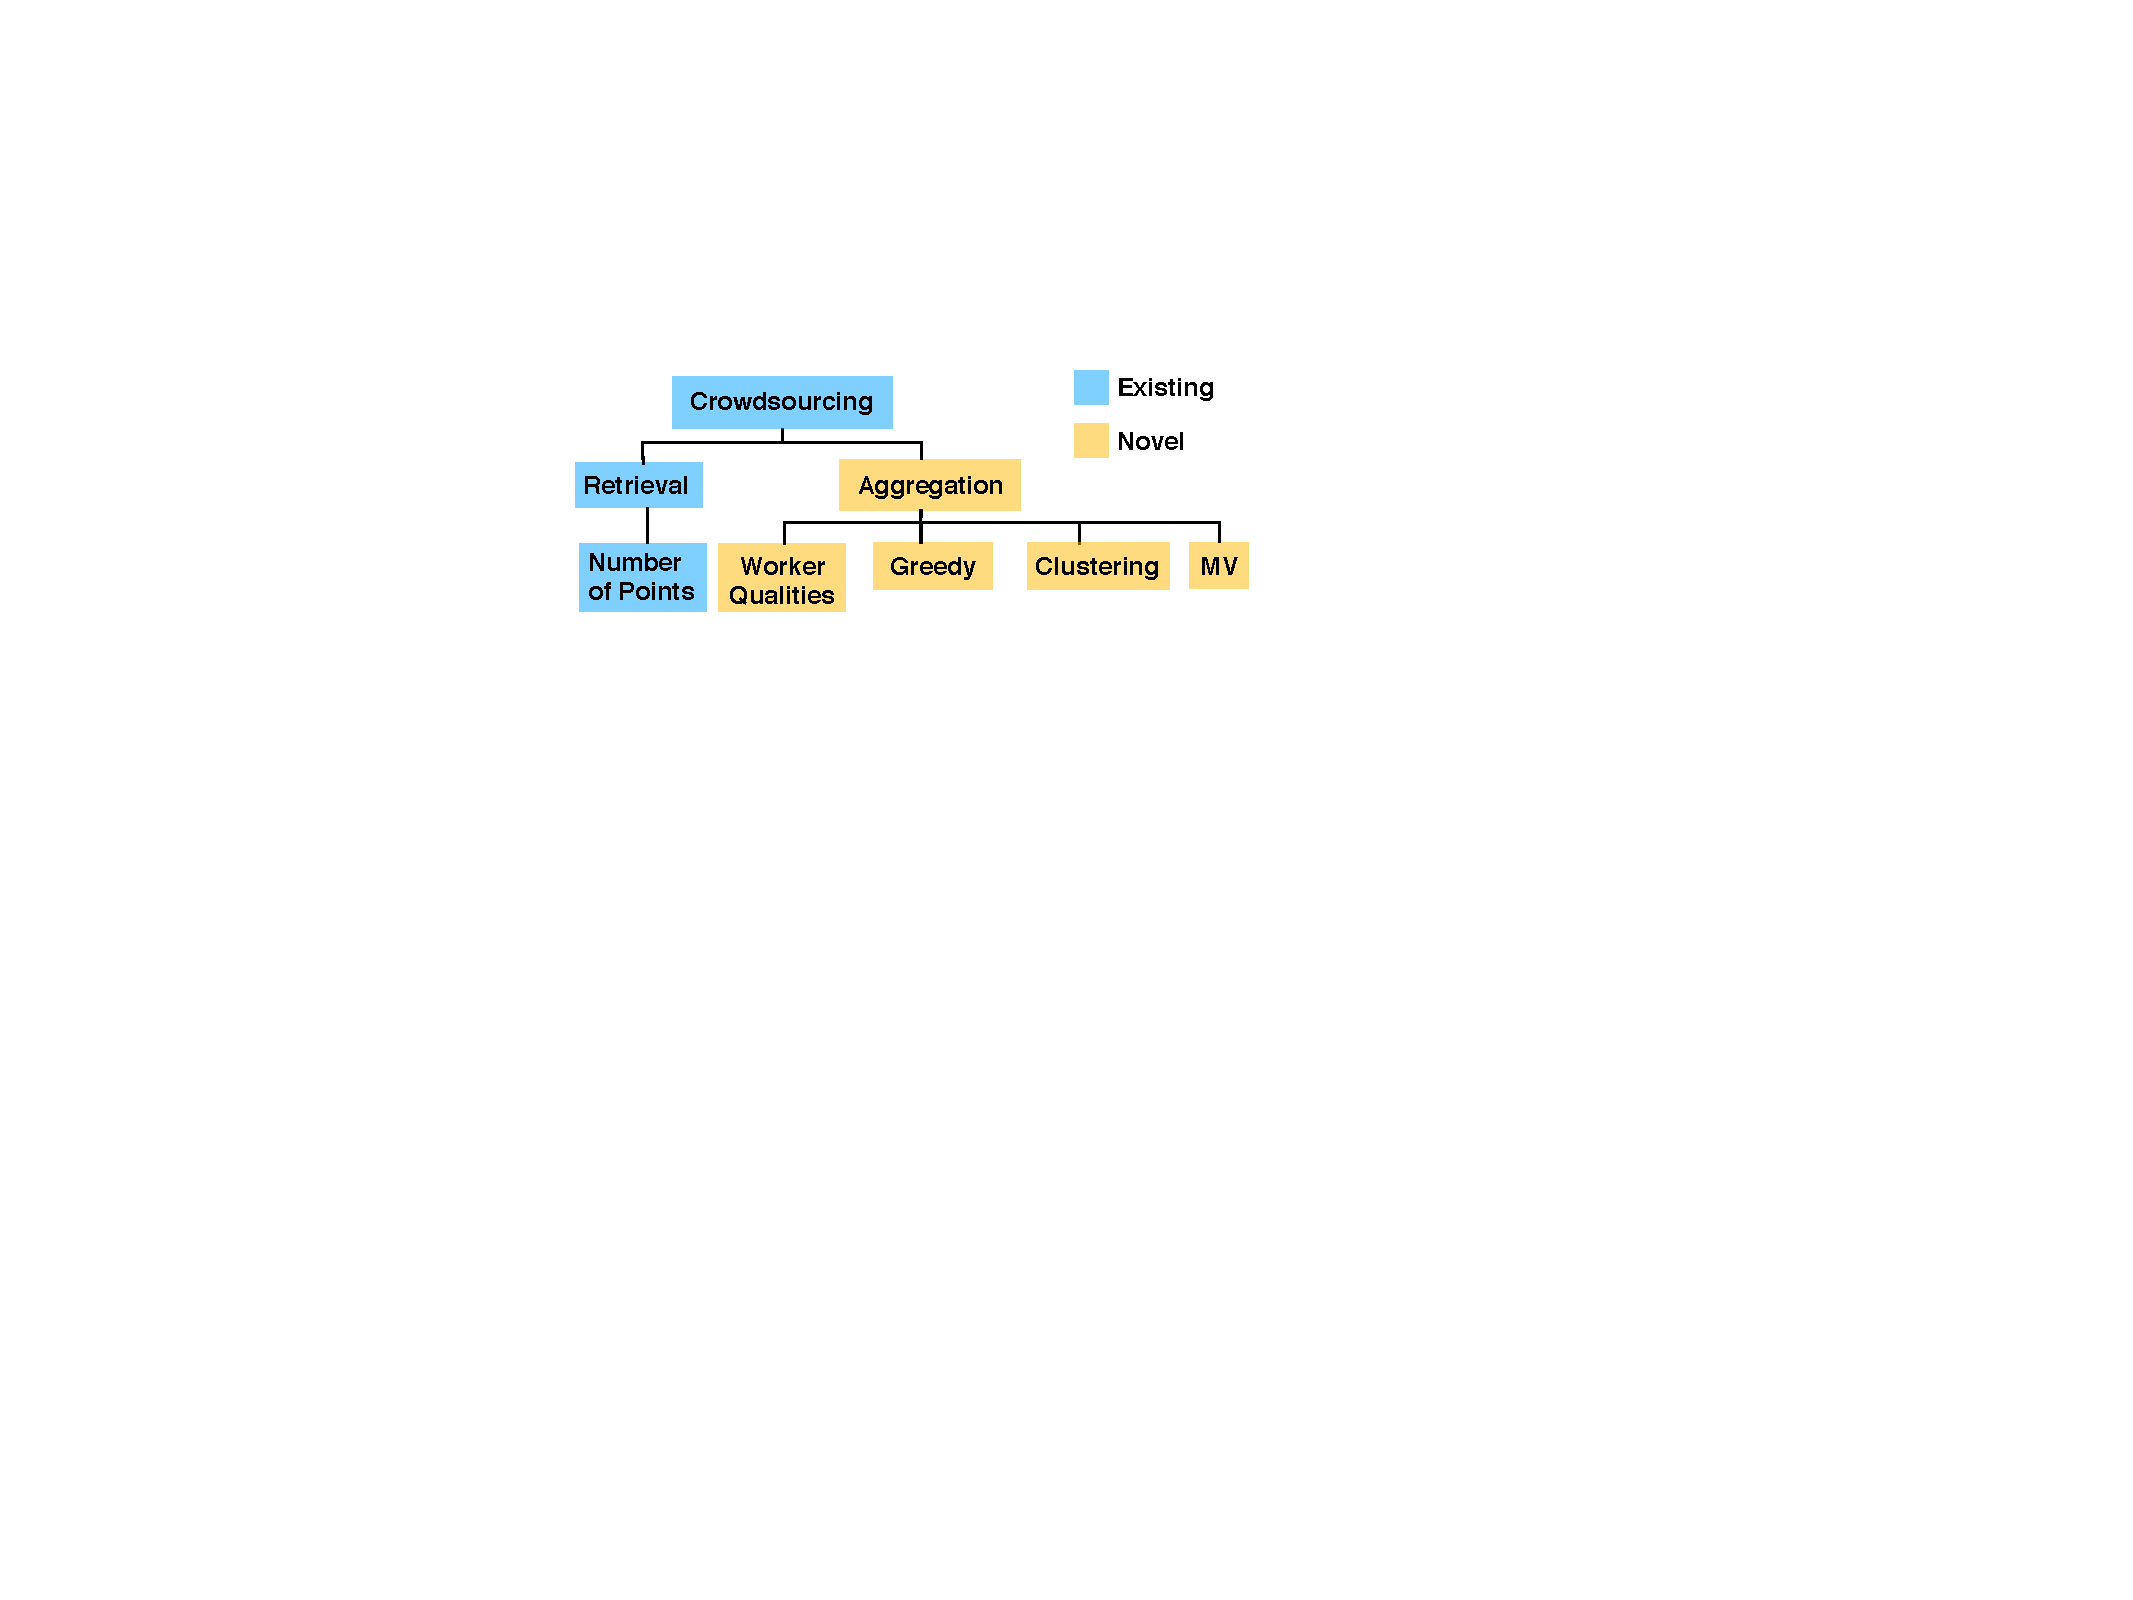
\includegraphics[width=0.75\linewidth]{plots/flowchart.pdf}
\caption{Taxonomy of quality evaluation algorithms for crowdsourced segmentation, including existing methods (blue) and a novel class of algorithms proposed in this paper (yellow).\vspace{-15pt}} %Majority-vote (MV) is colored both blue and yellow, since a common algorithm in crowdsourcing literature, but have not been extensively applied to crowdsourced image segmentation.}
%The crowdsourced approach can be largely classified as retrieval or aggregation-based methods. We further explore hybrid algorithms that makes use of signals that span over multiple categories, described in our technical report.
\label{flowchart}
% \setlength{\belowcaptionskip}{-30pt}
% \setlength{\abovecaptionskip}{-5pt} 
\end{figure}
%Many large-scale efforts in crowdsourced image segmentation contain little to no information on the quality characterization and evaluation of the collected dataset~\cite{Torralba2010,MartinFTM01,Li2009,Gurari2015}, which in dicate the lack of standardized approaches for quality evaluation. 
As shown in Figure~\ref{flowchart}, quality evaluation methods for crowdsourced segmentation can be classified into two categories:

\stitle{Retrieval-based methods} pick the ``best'' worker segmentation based on some scoring criteria that evaluates the quality of each segmentation, including vision information~\cite{Vittayakorn2011,Russakovsky2015}, and click-stream behavior \cite{Cabezas2015,Sameki2015,Sorokin2008}.

\stitle{Aggregation-based methods} combine multiple worker segmentations to produce a final segmentation that is not restricted to any single worker segmentation. An aggregation-based majority vote approach was employed in Sameki et al.~\cite{Sameki2015} to create an expert-established gold standard for characterizing their dataset and algorithmic accuracies, rather than for segmentation quality evaluation as described here.
%specialized segmentation interfaces or workflows that ensures that the annotations collected are of high quality, including 

\stitle{Vision-based methods} There has been a lot of prior work in segmenting objects based on color boundaries\cite{felzenszwalb2004efficient,Y.Y.Boykov2001}. These approaches, however, are typically non-exact, and far from robust. Furthermore, while they segment the entire image into several disjoint pieces, they do not serve to identify objects. Another class of prior works aim to segment specific semantic objects for objects of a specified type (e.g. cars, people)\cite{AdrianaKovashka2016,Lin2014,zhou2017scene}. Object segmentation using purely automated techniques would require training computer vision models on specific object types. 

\par Orthogonal methods to improve segmentation quality include periodic verification~\cite{Lin2014,Everingham15}, specialized interfaces~\cite{Song2018}, and vision-based supervision~\cite{Russakovsky2015,Gurari2016}. These methods could be used for quality improvement on top of any of the algorithms in this paper.  Since these policy-based methods are often interface-dependent or require expensive expert-drawn ground-truth annotations or vision information, their results are not easily reproducible. %In addition, the segmentations collected by the simple click-and-draw interface in many of the large scale segmentation efforts can not be improved with this technique as a post-processing method. Due to the lack of reproducibility, our paper do not compare against these policy-based methods in extensive details.
